\section*{Chapter 5}

\subsection*{Exercise 5.1}

$f: \mathbb{R}^3 \to \mathbb{R}^3$. $D_f = \begin{bmatrix} 3 & 1 & 1 \\ 0 & e^yz & e^y \\ yz & xz & xy \end{bmatrix}$

\subsection*{Exercise 5.2}

\begin{minipage}{0.45\linewidth}
    \begin{center}
        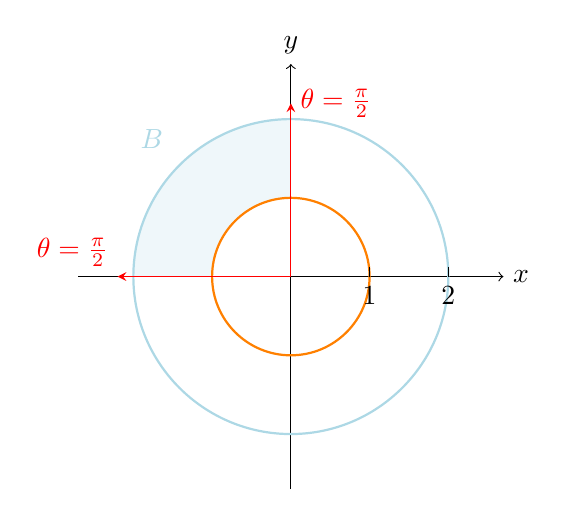
\begin{tikzpicture}
            \fill[LightBlue,fill opacity=0.2] (0,0) -- (180:2) arc (180:90:2) -- cycle;
            \fill[white,] (0,0) -- (180:1) arc (180:90:1) -- cycle;
            
            \draw[->] (-2.7,0) -- (2.7,0) node[right] {$x$};
            \draw[->] (0,-2.7) -- (0,2.7) node[above] {$y$};
            
            \draw[thick,LightBlue] (0,0) circle (2);
            \draw[thick,orange] (0,0) circle (1);
            
            \node[LightBlue,above left] at (-1.5,1.5) {$B$};
            
            \draw[red,-stealth] (0,0) -- (0,2.2) node[right] {$\theta=\frac{\pi}{2}$};
            \draw[red,-stealth] (0,0) -- (-2.2,0) node[above left] {$\theta=\frac{\pi}{2}$};
            \draw (1,0.125) -- (1,0) node[below] {$1$};
            \draw (2,0.125) -- (2,0) node[below] {$2$};
        \end{tikzpicture}
    \end{center}
\end{minipage}
$\overset{g}{\longrightarrow}$
\begin{minipage}{0.45\linewidth}
    \begin{center}
        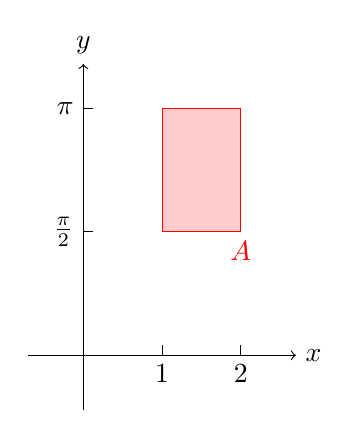
\begin{tikzpicture}
            \draw[->] (-0.7,0) -- (2.7,0) node[right] {$x$};
            \draw[->] (0,-0.7) -- (0,3.7) node[above] {$y$};
            
            \draw[red,fill=red,fill opacity=0.2] (1,1.57) -- (1,3.14) -- (2,3.14) -- (2,1.57) -- cycle;
            
            \draw (0.125,1.57) -- (0,1.57) node[left] {$\frac{\pi}{2}$};
            \draw (0.125,3.14) -- (0,3.14) node[left] {$\pi$};
            
            \draw (1,0.125) -- (1,0) node[below] {$1$};
            \draw (2,0.125) -- (2,0) node[below] {$2$};
            
            \node[red,below] at (2,1.57) {$A$};
        \end{tikzpicture}
    \end{center}
\end{minipage}

$\begin{aligned}
    \int_B x \,dA 
    &= \int_A r \cos{\theta} \cdot r \,dA \\
    &= \int_{r=1}^{r=2} \int_{\theta=\frac{\pi}{2}}^{\theta=\pi} r^2 \cos{\theta} \,d\theta \,dr
\end{aligned}$

\subsection*{Exercise 5.3}

$\begin{aligned}[t]
    \int_B x
     & = \int_A x \color{red} \cdot r                                                                             \\
     & = \int_{r=1}^{r=2} \int_{\theta=\frac{\pi}{2}}^{\theta=\pi} r \cos{\theta} \cdot r \,d\theta \,dr          \\
     & = \int_{r=1}^{r=2} r^2 \left( \int_{\theta=\frac{\pi}{2}}^{\theta=\pi} \cos{\theta} \,d\theta \right) \,dr \\
     & = \left( \int_{r=1}^{r=2} r^2 \,dr \right) \cdot\left( \int_{\theta=\frac{\pi}{2}}^{\theta=\pi} \cos{\theta} \,d\theta \right) \\
     & = \frac{r^3}{3} \bigg|_1^2 \cdot \sin{\theta} \bigg|_{\frac{\pi}{2}}^\pi                                   \\
     & = -\frac{7}{3}

% $\int_B x = \int_A x \cdot r = \int_{r=1}^{r=2} \int_{\theta=\frac{\pi}{2}}^{\theta=\pi} r \cos{\theta} \cdot r \,d\theta \,dr = \int_{r=1}^{r=2} r^2 \left( \int_{\theta}$ %TODO: finish me